


\tikzset{every picture/.style={line width=0.75pt}} %set default line width to 0.75pt        

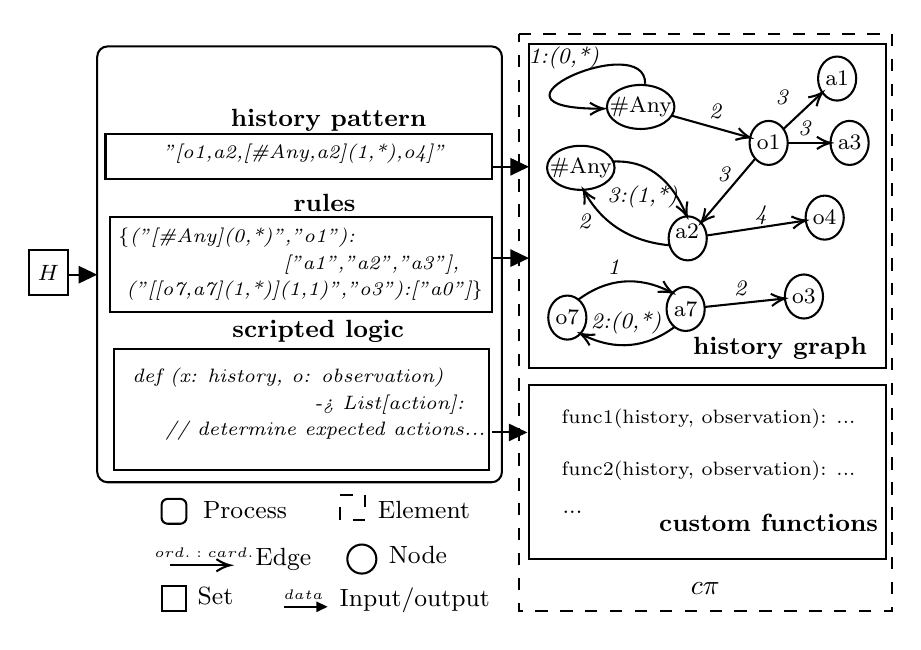
\begin{tikzpicture}[x=0.75pt,y=0.75pt,yscale=-1,xscale=1]
%uncomment if require: \path (0,1800); %set diagram left start at 0, and has height of 1800

%Shape: Rectangle [id:dp5530653457145052] 
\draw   (357,1533) -- (529,1533) -- (529,1617) -- (357,1617) -- cycle ;
%Curve Lines [id:da372228469894915] 
\draw    (413,1388) .. controls (413.41,1361.5) and (325.07,1400.34) .. (391.98,1400.01) ;
\draw [shift={(393,1400)}, rotate = 179.39] [color={rgb, 255:red, 0; green, 0; blue, 0 }  ][line width=0.75]    (6.56,-2.94) .. controls (4.17,-1.38) and (1.99,-0.4) .. (0,0) .. controls (1.99,0.4) and (4.17,1.38) .. (6.56,2.94)   ;
%Shape: Rectangle [id:dp19562386013401345] 
\draw  [dash pattern={on 4.5pt off 4.5pt}] (352,1364) -- (532,1364) -- (532,1642) -- (352,1642) -- cycle ;
%Straight Lines [id:da32046857444986476] 
\draw    (135,1480) -- (146,1480) ;
\draw [shift={(149,1480)}, rotate = 180] [fill={rgb, 255:red, 0; green, 0; blue, 0 }  ][line width=0.08]  [draw opacity=0] (8.93,-4.29) -- (0,0) -- (8.93,4.29) -- cycle    ;
%Shape: Rectangle [id:dp2045988237932408] 
\draw   (149,1375) .. controls (149,1372.24) and (151.24,1370) .. (154,1370) -- (339,1370) .. controls (341.76,1370) and (344,1372.24) .. (344,1375) -- (344,1575) .. controls (344,1577.76) and (341.76,1580) .. (339,1580) -- (154,1580) .. controls (151.24,1580) and (149,1577.76) .. (149,1575) -- cycle ;
%Straight Lines [id:da5454633151128134] 
\draw    (339.78,1428) -- (354,1428) ;
\draw [shift={(357,1428)}, rotate = 180] [fill={rgb, 255:red, 0; green, 0; blue, 0 }  ][line width=0.08]  [draw opacity=0] (8.93,-4.29) -- (0,0) -- (8.93,4.29) -- cycle    ;
%Straight Lines [id:da8020276364734138] 
\draw    (339.78,1472) -- (354,1472) ;
\draw [shift={(357,1472)}, rotate = 180] [fill={rgb, 255:red, 0; green, 0; blue, 0 }  ][line width=0.08]  [draw opacity=0] (8.93,-4.29) -- (0,0) -- (8.93,4.29) -- cycle    ;
%Shape: Rectangle [id:dp1935715039709336] 
\draw   (357,1369) -- (529,1369) -- (529,1525) -- (357,1525) -- cycle ;
%Shape: Rectangle [id:dp9576242016535905] 
\draw  [fill={rgb, 255:red, 255; green, 255; blue, 255 }  ,fill opacity=1 ] (180,1630) -- (192,1630) -- (192,1642) -- (180,1642) -- cycle ;
%Straight Lines [id:da5106599657188162] 
\draw    (239,1640) -- (257,1640) ;
\draw [shift={(260,1640)}, rotate = 180] [fill={rgb, 255:red, 0; green, 0; blue, 0 }  ][line width=0.08]  [draw opacity=0] (5.36,-2.57) -- (0,0) -- (5.36,2.57) -- cycle    ;
%Shape: Rectangle [id:dp11953132274699119] 
\draw  [fill={rgb, 255:red, 255; green, 255; blue, 255 }  ,fill opacity=1 ] (180,1591) .. controls (180,1589.34) and (181.34,1588) .. (183,1588) -- (189,1588) .. controls (190.66,1588) and (192,1589.34) .. (192,1591) -- (192,1597) .. controls (192,1598.66) and (190.66,1600) .. (189,1600) -- (183,1600) .. controls (181.34,1600) and (180,1598.66) .. (180,1597) -- cycle ;
%Shape: Rectangle [id:dp8011215111273835] 
\draw  [fill={rgb, 255:red, 255; green, 255; blue, 255 }  ,fill opacity=1 ][dash pattern={on 4.5pt off 4.5pt}] (266,1586) -- (278,1586) -- (278,1598) -- (266,1598) -- cycle ;
%Straight Lines [id:da8755027296416378] 
\draw    (184,1620) -- (211,1620) ;
\draw [shift={(213,1620)}, rotate = 180] [color={rgb, 255:red, 0; green, 0; blue, 0 }  ][line width=0.75]    (6.56,-2.94) .. controls (4.17,-1.38) and (1.99,-0.4) .. (0,0) .. controls (1.99,0.4) and (4.17,1.38) .. (6.56,2.94)   ;
%Shape: Circle [id:dp44369737646876817] 
\draw   (269.5,1617) .. controls (269.5,1613.13) and (272.63,1610) .. (276.5,1610) .. controls (280.37,1610) and (283.5,1613.13) .. (283.5,1617) .. controls (283.5,1620.87) and (280.37,1624) .. (276.5,1624) .. controls (272.63,1624) and (269.5,1620.87) .. (269.5,1617) -- cycle ;
%Straight Lines [id:da30661950995273646] 
\draw    (339,1556) -- (353.22,1556) ;
\draw [shift={(356.22,1556)}, rotate = 180] [fill={rgb, 255:red, 0; green, 0; blue, 0 }  ][line width=0.08]  [draw opacity=0] (8.93,-4.29) -- (0,0) -- (8.93,4.29) -- cycle    ;
%Shape: Rectangle [id:dp04589846178831558] 
\draw   (153,1412) -- (339,1412) -- (339,1434) -- (153,1434) -- cycle ;
%Shape: Rectangle [id:dp10989145637614484] 
\draw   (155.04,1452) -- (339,1452) -- (339,1498) -- (155.04,1498) -- cycle ;
%Shape: Rectangle [id:dp013048181643078749] 
\draw   (157.09,1516) -- (337.98,1516) -- (337.98,1574) -- (157.09,1574) -- cycle ;


% Text Node
\draw (378,1594.5) node  [font=\footnotesize,color={rgb, 255:red, 0; green, 0; blue, 0 }  ,opacity=1 ] [align=left] {...};
% Text Node
\draw (443.5,1574.5) node  [font=\footnotesize,color={rgb, 255:red, 0; green, 0; blue, 0 }  ,opacity=1 ] [align=left] {{\scriptsize func2(history, observation): ...}};
% Text Node
\draw (303,1613) node  [font=\footnotesize] [align=left] {\begin{minipage}[lt]{20.27pt}\setlength\topsep{0pt}
\begin{center}
{\small Node}
\end{center}

\end{minipage}};
% Text Node
\draw (200.5,1614) node  [font=\tiny] [align=left] {$ord.:card.$};
% Text Node
\draw (238.5,1615) node  [font=\footnotesize] [align=left] {\begin{minipage}[lt]{19.87pt}\setlength\topsep{0pt}
\begin{center}
{\small Edge}
\end{center}

\end{minipage}};
% Text Node
\draw (304,1591) node  [font=\footnotesize] [align=left] {\begin{minipage}[lt]{29.65pt}\setlength\topsep{0pt}
\begin{center}
{\small Element}
\end{center}

\end{minipage}};
% Text Node
\draw (251,1542.5) node  [font=\footnotesize,color={rgb, 255:red, 0; green, 0; blue, 0 }  ,opacity=1 ] [align=left] {{\scriptsize \textit{def (x: history, o: observation)}}\\{\scriptsize \textit{ \ \ \ \ \ \ \ \ \ \ \ \ \ \ \ \ \ \ \ \ \ -> List[action]:}}\\{\scriptsize \textit{ \ \ \ // determine expected actions... }}};
% Text Node
\draw (443.5,1549.5) node  [font=\footnotesize,color={rgb, 255:red, 0; green, 0; blue, 0 }  ,opacity=1 ] [align=left] {{\scriptsize func1(history, observation): ...}};
% Text Node
\draw (472.5,1599.5) node  [font=\small] [align=left] {{\small \textbf{custom functions}}};
% Text Node
\draw (469.5,1451.5) node  [font=\scriptsize] [align=left] {{\footnotesize \textit{4}}};
% Text Node
\draw (412,1442.5) node  [font=\scriptsize] [align=left] {{\footnotesize \textit{3:(1,*)}}};
% Text Node
\draw (384.5,1454.5) node  [font=\scriptsize] [align=left] {{\footnotesize \textit{2}}};
% Text Node
\draw    (499.5, 1452.5) circle [x radius= 9.19, y radius= 10.61]   ;
\draw (499.5,1452.5) node  [font=\scriptsize] [align=left] {{\footnotesize o4}};
% Text Node
\draw    (382, 1428.5) circle [x radius= 16.26, y radius= 10.61]   ;
\draw (382,1428.5) node  [font=\scriptsize] [align=left] {{\footnotesize \#Any}};
% Text Node
\draw    (433.5, 1462.5) circle [x radius= 9.19, y radius= 10.61]   ;
\draw (426,1454) node [anchor=north west][inner sep=0.75pt]  [font=\scriptsize] [align=left] {{\footnotesize a2}};
% Text Node
\draw (490.5,1409.5) node  [font=\scriptsize] [align=left] {{\footnotesize \textit{3}}};
% Text Node
\draw (451.5,1431.5) node  [font=\scriptsize] [align=left] {{\footnotesize \textit{3}}};
% Text Node
\draw (479.5,1394.5) node  [font=\scriptsize] [align=left] {{\footnotesize \textit{3}}};
% Text Node
\draw (447.5,1401.5) node  [font=\scriptsize] [align=left] {{\footnotesize \textit{2}}};
% Text Node
\draw (374,1375.5) node  [font=\scriptsize] [align=left] {{\footnotesize \textit{1:(0,*)}}};
% Text Node
\draw    (511.5, 1416.5) circle [x radius= 9.19, y radius= 10.61]   ;
\draw (511.5,1416.5) node  [font=\scriptsize] [align=left] {{\footnotesize a3}};
% Text Node
\draw    (505.5, 1385.5) circle [x radius= 9.19, y radius= 10.61]   ;
\draw (505.5,1385.5) node  [font=\scriptsize] [align=left] {{\footnotesize a1}};
% Text Node
\draw    (472.5, 1416.5) circle [x radius= 9.19, y radius= 10.61]   ;
\draw (472.5,1416.5) node  [font=\scriptsize] [align=left] {{\footnotesize o1}};
% Text Node
\draw    (410.84, 1399.18) circle [x radius= 16.26, y radius= 10.61]   ;
\draw (410.84,1399.18) node  [font=\scriptsize] [align=left] {{\footnotesize \#Any}};
% Text Node
\draw    (116,1468) -- (135,1468) -- (135,1490) -- (116,1490) -- cycle  ;
\draw (125.5,1479) node  [font=\footnotesize] [align=left] {$\displaystyle H$};
% Text Node
\draw (260.5,1385) node  [font=\normalsize] [align=left] {$\displaystyle $};
% Text Node
\draw (478,1515.5) node  [font=\small] [align=left] {{\small \textbf{history graph}}};
% Text Node
\draw (442,1631) node  [font=\normalsize] [align=left] {$\displaystyle c\pi $};
% Text Node
\draw (459.5,1486.5) node  [font=\scriptsize] [align=left] {{\footnotesize \textit{2}}};
% Text Node
\draw (404,1503.5) node  [font=\scriptsize] [align=left] {{\footnotesize \textit{2:(0,*)}}};
% Text Node
\draw (398.5,1476.5) node  [font=\scriptsize] [align=left] {{\footnotesize \textit{1}}};
% Text Node
\draw    (489.5, 1490.5) circle [x radius= 9.19, y radius= 10.61]   ;
\draw (489.5,1490.5) node  [font=\scriptsize] [align=left] {{\footnotesize o3}};
% Text Node
\draw    (432.5, 1496.5) circle [x radius= 9.19, y radius= 10.61]   ;
\draw (432.5,1496.5) node  [font=\scriptsize] [align=left] {{\footnotesize a7}};
% Text Node
\draw    (375.5, 1500.66) circle [x radius= 9.19, y radius= 10.61]   ;
\draw (375.5,1500.66) node  [font=\scriptsize] [align=left] {{\footnotesize o7}};
% Text Node
\draw (247.02,1475) node  [font=\footnotesize] [align=left] {{\scriptsize \textit{\{("[\#Any](0,*)","o1"):}}\\{\scriptsize \textit{ \ \ \ \ \ \ \ \ \ \ \ \ \ \ \ \ \ \ \ ["a1","a2","a3"],}}\\{\scriptsize \textit{ ("[[o7,a7](1,*)](1,1)","o3"):["a0"]\}}}};
% Text Node
\draw (255.5,1507.5) node  [font=\small] [align=left] {{\small \textbf{scripted logic}}};
% Text Node
\draw (258.5,1445.5) node  [font=\small] [align=left] {{\small \textbf{rules}}};
% Text Node
\draw (249,1421.5) node  [font=\footnotesize] [align=left] {{\scriptsize \textit{"[o1,a2,[\#Any,a2](1,*),o4]"}}};
% Text Node
\draw (260.5,1405.5) node  [font=\small] [align=left] {{\small \textbf{history pattern}}};
% Text Node
\draw (219.5,1591) node  [font=\footnotesize] [align=left] {\begin{minipage}[lt]{29.25pt}\setlength\topsep{0pt}
\begin{center}
{\small Process}
\end{center}

\end{minipage}};
% Text Node
\draw (248.5,1634) node  [font=\tiny] [align=left] {$data$};
% Text Node
\draw (293.5,1635) node  [font=\footnotesize] [align=left] {\begin{minipage}[lt]{41.51pt}\setlength\topsep{0pt}
\begin{center}
{\small Input/output}
\end{center}

\end{minipage}};
% Text Node
\draw (206,1635) node  [font=\footnotesize] [align=left] {\begin{minipage}[lt]{13.75pt}\setlength\topsep{0pt}
\begin{center}
{\small Set}
\end{center}

\end{minipage}};
% Connection
\draw    (442.62,1461.12) -- (488.41,1454.18) ;
\draw [shift={(490.38,1453.88)}, rotate = 171.38] [color={rgb, 255:red, 0; green, 0; blue, 0 }  ][line width=0.75]    (6.56,-2.94) .. controls (4.17,-1.38) and (1.99,-0.4) .. (0,0) .. controls (1.99,0.4) and (4.17,1.38) .. (6.56,2.94)   ;
% Connection
\draw    (397.6,1425.48) .. controls (413.2,1424.74) and (424.82,1433.01) .. (432.44,1450.27) ;
\draw [shift={(433.14,1451.9)}, rotate = 247.5] [color={rgb, 255:red, 0; green, 0; blue, 0 }  ][line width=0.75]    (6.56,-2.94) .. controls (4.17,-1.38) and (1.99,-0.4) .. (0,0) .. controls (1.99,0.4) and (4.17,1.38) .. (6.56,2.94)   ;
% Connection
\draw    (424.77,1465.83) .. controls (406.35,1464.06) and (392.81,1455.71) .. (384.13,1440.73) ;
\draw [shift={(383.2,1439.08)}, rotate = 61.69] [color={rgb, 255:red, 0; green, 0; blue, 0 }  ][line width=0.75]    (6.56,-2.94) .. controls (4.17,-1.38) and (1.99,-0.4) .. (0,0) .. controls (1.99,0.4) and (4.17,1.38) .. (6.56,2.94)   ;
% Connection
\draw    (466.07,1424.08) -- (441.22,1453.39) ;
\draw [shift={(439.93,1454.92)}, rotate = 310.29] [color={rgb, 255:red, 0; green, 0; blue, 0 }  ][line width=0.75]    (6.56,-2.94) .. controls (4.17,-1.38) and (1.99,-0.4) .. (0,0) .. controls (1.99,0.4) and (4.17,1.38) .. (6.56,2.94)   ;
% Connection
\draw    (481.69,1416.5) -- (500.31,1416.5) ;
\draw [shift={(502.31,1416.5)}, rotate = 180] [color={rgb, 255:red, 0; green, 0; blue, 0 }  ][line width=0.75]    (6.56,-2.94) .. controls (4.17,-1.38) and (1.99,-0.4) .. (0,0) .. controls (1.99,0.4) and (4.17,1.38) .. (6.56,2.94)   ;
% Connection
\draw    (479.63,1409.8) -- (496.91,1393.57) ;
\draw [shift={(498.37,1392.2)}, rotate = 136.79] [color={rgb, 255:red, 0; green, 0; blue, 0 }  ][line width=0.75]    (6.56,-2.94) .. controls (4.17,-1.38) and (1.99,-0.4) .. (0,0) .. controls (1.99,0.4) and (4.17,1.38) .. (6.56,2.94)   ;
% Connection
\draw    (425.78,1403.37) -- (461.64,1413.45) ;
\draw [shift={(463.57,1413.99)}, rotate = 195.69] [color={rgb, 255:red, 0; green, 0; blue, 0 }  ][line width=0.75]    (6.56,-2.94) .. controls (4.17,-1.38) and (1.99,-0.4) .. (0,0) .. controls (1.99,0.4) and (4.17,1.38) .. (6.56,2.94)   ;
% Connection
\draw    (441.65,1495.54) -- (478.36,1491.67) ;
\draw [shift={(480.35,1491.46)}, rotate = 173.99] [color={rgb, 255:red, 0; green, 0; blue, 0 }  ][line width=0.75]    (6.56,-2.94) .. controls (4.17,-1.38) and (1.99,-0.4) .. (0,0) .. controls (1.99,0.4) and (4.17,1.38) .. (6.56,2.94)   ;
% Connection
\draw    (427.19,1505.16) .. controls (413.32,1515.36) and (398.76,1516.72) .. (383.47,1509.23) ;
\draw [shift={(381.81,1508.38)}, rotate = 27.94] [color={rgb, 255:red, 0; green, 0; blue, 0 }  ][line width=0.75]    (6.56,-2.94) .. controls (4.17,-1.38) and (1.99,-0.4) .. (0,0) .. controls (1.99,0.4) and (4.17,1.38) .. (6.56,2.94)   ;
% Connection
\draw    (380.81,1492) .. controls (394.68,1481.8) and (409.24,1480.44) .. (424.53,1487.93) ;
\draw [shift={(426.19,1488.78)}, rotate = 207.94] [color={rgb, 255:red, 0; green, 0; blue, 0 }  ][line width=0.75]    (6.56,-2.94) .. controls (4.17,-1.38) and (1.99,-0.4) .. (0,0) .. controls (1.99,0.4) and (4.17,1.38) .. (6.56,2.94)   ;

\end{tikzpicture}